\chapter{Pianificazione delle attività}

Il progetto consiste nel valutare da un punto di vista temporale i risultati degli esperimenti eseguiti con Snort. Per fare questo abbiamo utilizzato due macchine con OS Ubuntu 12.04 su cui, seguendo i passi descritti nel capito successivo, abbiamo installato e opportunamente configurato Snort come IDS. Il sistema alla base delle analisi quindi si compone di una prima macchina che avrà funzione di sistema da difendere (nodo A) ed una seconda con la funzione di attaccante (nodo B) collegate ad una rete wifi locale.
La necessità di eseguire Snort su entrambe le componenti del sistema è legata alla necessità di dover tracciare i tempi d'invio, d'iniezione e d'individuazione delle operazioni di fault injection. In pratica, nel nodo A Snort provvederà sia a loggare tutto il traffico diretto verso se stesso dal nodo B, sia a generare gli alert dovuti agli attacchi individuati, mentre nel nodo B provvederà a loggare tutti i pacchetti diretti da B ad A, così da tracciare i tempi d'invio degli attacchi. I codici relativi alle regole Snort che sono state scritte per permettere ai due nodi di fare sia da Packet Sniffer che da Packet Logger possono essere trovati nell'Appendice A, Codici \ref{lst:attaccante} e \ref{lst:ids}.\\
Il sistema di misura si compone quindi dei due file di log generati rispettivamente sui due nodi che, assieme all'output dei software usati per generare la fault injection, permettono di registrare tutta la storia temporale degli attacchi al fine di verificare l'azione delle regole di Snort.\\
Purtroppo, in un primo momento di analisi del problema e di sperimentazione, ritenevamo sufficiente loggare soltanto i pacchetti in entrata ed in uscita, rispettivamente, nel nodo A e dal nodo B. Soltanto in fase di analisi ci siamo resi conto che, senza il flusso di dati in entrambe le direzioni ed in entrambi i nodi, alcune misure (come ad esempio la durata totale dell'attacco) non potevano essere calcolate correttamente. Per ragioni di tempistiche, abbiamo deciso di mantenere gli esperimenti e i relativi log così com'erano, precisando comunque che alcune misure, per questo motivo, sono state approssimate e consci del fatto che un'applicazione più rigida della metodologia di testing avrebbe richiesto la ripetizione di tutti gli esperimenti con le nuove specifiche.

\begin{figure}[h!]
	\centering
	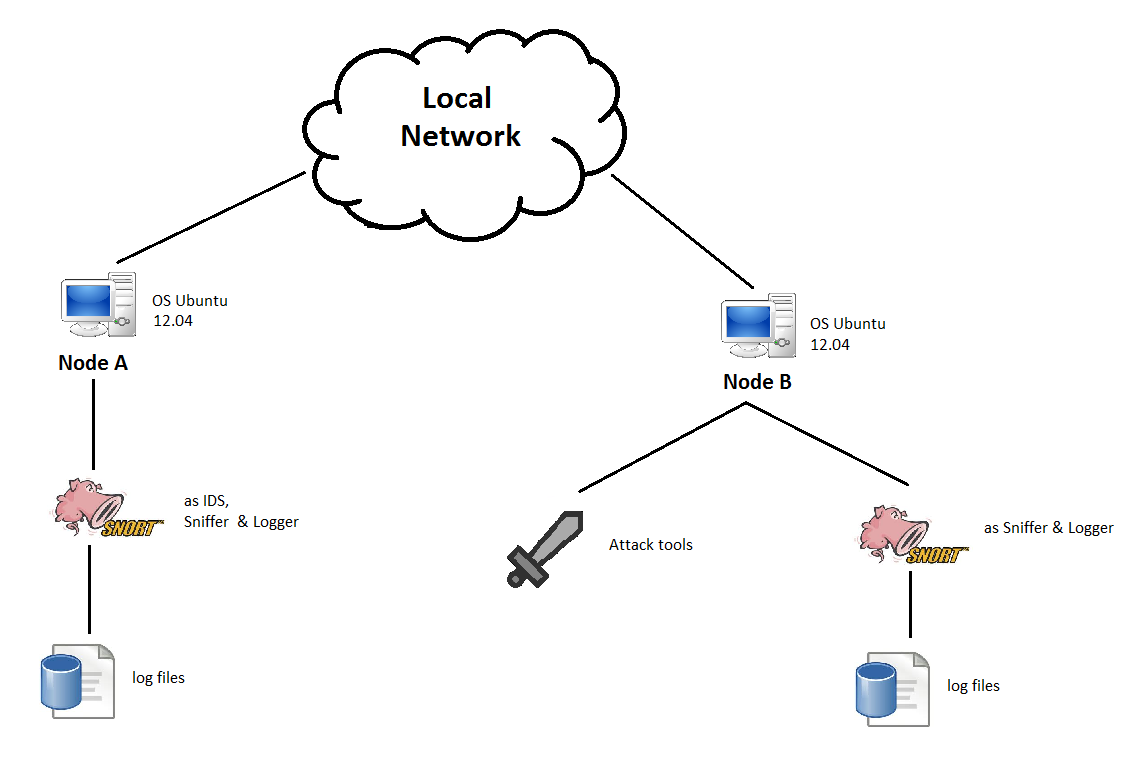
\includegraphics[scale=0.5]{figure/schema.png}
	\caption{Schema della configurazione utilizzata nei vari esperimenti.}
\end{figure}

\section{Sfasamento dei clock}

Il ``semplice'' sistema di misura brevemente descritto in precedenza deve però tenere conto del problema dello sfasamento dei clock sulle due macchine, è infatti errato assumere che entrambe abbiano la stessa visione del tempo che è appunto governata dal clock interno a ciascuna macchina. Inoltre, anche se in un certo istante il clock delle due macchine segnasse lo stesso valore, non è detto che questo valga sempre: è infatti possibile che i due clock si allontanino o si avvicinino durante il tempo, rendendo impossibile fare qualsiasi stima di natura statica.\\
Per fare sì che i tempi registrati nel nodo A siano consistenti a quelli registrati nel nodo B è necessario mettere in piedi un processo di sincronizzazione. Un protocollo utile per, parzialmente, risolvere il problema è il Network Time Protocol, in sigla NTP, un protocollo per la sincronizzazione degli orologi di computer all'interno di una rete a commutazione di pacchetto.\\
Come prima cosa quindi è necessario scaricare ed installare su entrambe le macchine il pacchetto \textit{ntp} che mette a disposizione varie funzionalità per la sincronizzazione.\\
Un primo approccio può fare uso del comando \textbf{ntpd}, il quale mette in esecuzione un processo \textit{demone} che in \textit{background} provvede a sincronizzare l'orologio di sistema con quello di un server opportunamente specificato nel file (\textit{/etc/ntp.conf}). Questo approccio ha però due problemi: richiede alcune ore per arrivare a registrare una buona approssimazione del tempo del server e continuando la sua esecuzione in background e in modo asincrono rispetto all'altra macchina che compone il sistema può andare a modificare la visione del tempo di una macchina durante l'esecuzione di un'esperimento rischiando di produrre inconsistenze tra i dati raccolti.
Per fornire evidenza di questa situazione riportiamo qui di seguito due frammenti di log relativi al nodo A e al nodo B durante un esperimento di fault injection (alcuni dettagli non rilevanti sono stati omessi per una maggiore chiarezza di lettura):

\begin{center}
	\textbf{Nodo A:}
	\begin{tabular}{|c|c|c|c|c|}
	\hline
	TIMESTAMP & MSG & PROTOCOL & FROM\_IP & TO\_IP\\
	\hline
	07/09-17:38:37.271491 & ICMP PING BSDtype&	ICMP&	192.168.137.170&		192.168.137.180\\
	\hline
	07/09-17:38:37.271491& 		ICMP PING *NIX&	ICMP&	192.168.137.170	&	192.168.137.180\\
	\hline
	07/09-17:38:37.271491 &	PACKET RECEIVED&	ICMP&	192.168.137.170&		192.168.137.180\\
	\hline
	07/09-17:38:37.271491 &	ICMP PING&	ICMP&	192.168.137.170&		192.168.137.180\\
	\hline
	07/09-17:38:37.271544&	ICMP Echo Reply&	ICMP&	192.168.137.180&		192.168.137.170\\
	\hline
	07/09-17:38:38.194984 &	ICMP PING BSDtype	& ICMP&	192.168.137.170&		192.168.137.180\\
	\hline
	07/09-17:38:38.194984 &	ICMP PING *NIX&	ICMP&	192.168.137.170&		192.168.137.180\\
	\hline
	07/09-17:38:38.194984 &	PACKET RECEIVED&	ICMP&	192.168.137.170&		192.168.137.180\\
	\hline
	07/09-17:38:38.194984 &	ICMP PING&	ICMP&	192.168.137.170&		192.168.137.180\\
	\hline
	07/09-17:38:38.195038 &	ICMP Echo Reply	& ICMP&	192.168.137.180&		192.168.137.170\\
	\hline
	07/09-17:38:39.116375 &	ICMP PING BSDtype&	ICMP&	192.168.137.170&		192.168.137.180\\
	\hline
	07/09-17:38:39.116375 &	ICMP PING *NIX&	ICMP&	192.168.137.170&		192.168.137.180\\
	\hline
	07/09-17:38:39.116375 &	PACKET RECEIVED&	ICMP&	192.168.137.170&		192.168.137.180\\
	\hline
	07/09-17:38:39.116375 &	ICMP PING&	ICMP&	192.168.137.170&		192.168.137.180\\
	\hline
	07/09-17:38:39.116406 &	ICMP Echo Reply&	ICMP&	192.168.137.180&		192.168.137.170\\
	\hline
	07/09-17:38:40.140671 &	ICMP PING BSDtype&	ICMP&	192.168.137.170&		192.168.137.180\\
	\hline
	07/09-17:38:40.140671 &	ICMP PING *NIX&	ICMP&	192.168.137.170&		192.168.137.180\\
	\hline
	07/09-17:38:40.140671&	PACKET RECEIVED&	ICMP&	192.168.137.170	&	192.168.137.180\\
	\hline
	07/09-17:38:40.140671 &	ICMP PING&	ICMP&	192.168.137.170&		192.168.137.180\\
	\hline
	07/09-17:38:40.140727 &	ICMP Echo Reply&	ICMP&	192.168.137.180	&	192.168.137.170\\
	\hline
	07/09-17:38:47.513307 	&	PACKET RECEIVED&	TCP&	192.168.137.170&	192.168.137.180\\
	\hline
	\end{tabular}
\end{center}
\clearpage
\begin{center}
	\textbf{Nodo B:}
	\begin{tabular}{|c|c|c|c|c|}
	\hline
	TIMESTAMP & MSG & PROTOCOL & FROM\_IP & TO\_IP\\
	\hline
	07/09-17:38:37.128073&	ICMP PING BSDtype&	ICMP&	192.168.137.170	&	192.168.137.180\\
		\hline
	07/09-17:38:37.128073 &	ICMP PING *NIX&	ICMP&	192.168.137.170	&	192.168.137.180\\
		\hline
	07/09-17:38:37.128073 &	PACKET SENT&	ICMP&	192.168.137.170	&	192.168.137.180\\
		\hline
	07/09-17:38:37.128073 &	ICMP PING&	ICMP&	192.168.137.170	&	192.168.137.180\\
		\hline
	07/09-17:38:37.320961 &	ICMP Echo Reply	& ICMP&	192.168.137.180	&	192.168.137.170\\
		\hline
	07/09-17:38:38.129178 &	ICMP PING BSDtype&	ICMP&	192.168.137.170&		192.168.137.180\\
		\hline
	07/09-17:38:38.129178 &	ICMP PING *NIX&	ICMP&	192.168.137.170	&	192.168.137.180\\
		\hline
	07/09-17:38:38.129178 &	PACKET SENT&	ICMP&	192.168.137.170	&	192.168.137.180\\
		\hline
	07/09-17:38:38.129178 &	ICMP PING&	ICMP&	192.168.137.170	&	192.168.137.180\\
		\hline
	07/09-17:38:38.243095 &	ICMP Echo Reply&	ICMP&	192.168.137.180	&	192.168.137.170\\
		\hline
	07/09-17:38:39.130354 &	ICMP PING BSDtype&	ICMP&	192.168.137.170&		192.168.137.180\\
		\hline
	07/09-17:38:39.130354 &	ICMP PING *NIX&	ICMP&	192.168.137.170&		192.168.137.180\\
		\hline
	07/09-17:38:39.130354 	&	PACKET SENT&	ICMP&	192.168.137.170	&	192.168.137.180\\
		\hline
	07/09-17:38:39.130354 	&	ICMP PING&	ICMP&	192.168.137.170	&	192.168.137.180\\
		\hline
	07/09-17:38:39.163513 &	ICMP Echo Reply&	ICMP&	192.168.137.180	&	192.168.137.170\\
		\hline
	07/09-17:38:40.131860 &	ICMP PING BSDtype&	ICMP&	192.168.137.170	&	192.168.137.180\\
		\hline
	07/09-17:38:40.131860 &	ICMP PING *NIX&	ICMP&	192.168.137.170	&	192.168.137.180\\
		\hline
	07/09-17:38:40.131860 &	PACKET SENT	& ICMP&	192.168.137.170&		192.168.137.180\\
		\hline
	07/09-17:38:40.131860 &	ICMP PING&	ICMP&	192.168.137.170	&	192.168.137.180\\
		\hline
	07/09-17:38:40.190195 	&	ICMP Echo Reply&	ICMP&	192.168.137.180	&	192.168.137.170\\
		\hline
	07/09-17:38:47.564978 &	PACKET SENT&	UDP&	192.168.137.170&	192.168.137.1\\
		\hline
	\end{tabular}
\end{center}

Osservando i tempi d'invio ed i tempi di recezione dei messaggi si può facilmente notare come per i primi pacchetti i tempi di recezione, come ci si può aspettare, siano maggiori dei tempi d'invio mentre questo non vale dal quinto pacchetto in poi dove i tempi di recezione risultano improvvisamente minori dei tempi d'invio. Questa inconsistenza può essere frutto di una sincronizzazione dell'orologio di una delle due macchine per mezzo del demone generato con il comando \textit{ntpd} o anche uno sfasamento dei clock. La possibilità d'occorrenza di questa situazione rende quindi impossibile dare confidenza sui risultati ottenuti a causa della variabilità della visione temporale, di una o di entrambe le macchine, durante l'esecuzione di un esperimento.\\
Questo problema può essere risolto utilizzando altri due comandi. Sarà infatti necessario disattiva il servizio \textit{ntp} eliminando il problema della sincronizzazione degli orologi asincrona tra le due macchine, utilizzando il comando \textit{service ntp stop}. Successivamente dopo l'esecuzione di ogni esperimento sarà necessario utilizzare il comando \textit{ntpdate}, il quale permette di sincronizzare l'orologio e ricevere l'offset di aggiustamento applicato. Utilizzando quest'offset che corrisponde ad una stima dell'errore temporale commesso da ciascuna macchina, durante l'esecuzione dell'esperimento, possiamo cercare di "correggere" le misure registrate. Ad esempio se l'offset resitutito da \textit{ntpdate} sul nodo A è +2ms mentre l'offset restituito sul nodo B è -4ms, si può cercare di correggere le misure registrate sul nodo A e sul nodo B rispettivamente sommando e sottraendo tali offset.
Questa correzione naturalmente non elimina totalmente l'errore sistematico commesso, in quanto gli offset sono stime dell'errore, ma si riesce comunque a limitare l'errore di misurazione.
Quindi il sistema di misura introdotto avrà come riferimento l'orologio (il clock) del server utilizzato con il comando \textit{ntpdate}, la procedura di misura consisterà nell'effettuare il \textit{timestamp} di ogni pacchetto inviato/ricevuto con una risoluzione di \textit{$10^{-6}$s} ed un'intrusività trascurabile per la risoluzione apprezzata. Ad ognuno di questi tempi sarà poi sommato/sottratto l'offset tra il tempo macchina e il tempo del server riscontrato durante l'esperimento.


